
\begin{figure}[H]
  {
    \setlength{\tabcolsep}{3.0pt}
    \setlength\cmidrulewidth{\heavyrulewidth} % Make cmidrule = 
    \begin{adjustbox}{height=5cm,center}
      \footnotesize
      \begin{tabular}{ll}

        \makecell[l]{
\icode{.BYTE \$FF,\$01}\\
\icode{.BYTE \$01,\$FF}
} & \makecell[l]{

\includegraphics[width=1.3cm]{src/patterns/pixels/pixel_pattern5_0.png}%
} \\
        \midrule

        \makecell[l]{
\icode{.BYTE \$FE,\$02}\\
\icode{.BYTE \$FE,\$02}
} & \makecell[l]{

\includegraphics[width=1.3cm]{src/patterns/pixels/pixel_pattern5_1.png}%

\includegraphics[width=1.3cm]{src/patterns/pixels/pixel_pattern5_2.png}%
} \\
        \midrule

        \makecell[l]{
\icode{.BYTE \$FD,\$03}\\
\icode{.BYTE \$03,\$FD}
} & \makecell[l]{
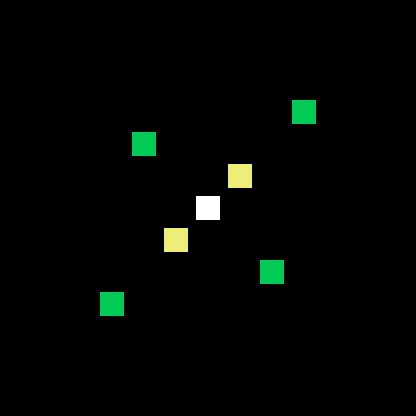
\includegraphics[width=1.3cm]{src/patterns/pixels/pixel_pattern5_3.png}%
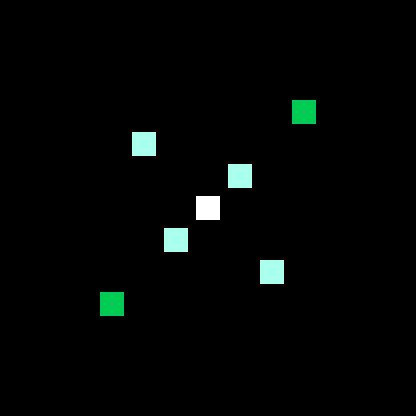
\includegraphics[width=1.3cm]{src/patterns/pixels/pixel_pattern5_4.png}%
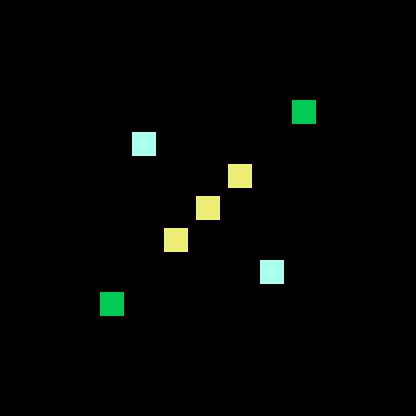
\includegraphics[width=1.3cm]{src/patterns/pixels/pixel_pattern5_5.png}%
} \\
        \midrule

        \makecell[l]{
\icode{.BYTE \$FC,\$04,\$FC,\$FC,\$04,\$04}\\
\icode{.BYTE \$FC,\$04,\$FF,\$01,\$FF,\$01}
} & \makecell[l]{
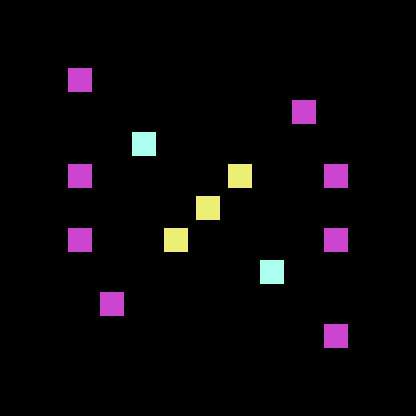
\includegraphics[width=1.3cm]{src/patterns/pixels/pixel_pattern5_6.png}%
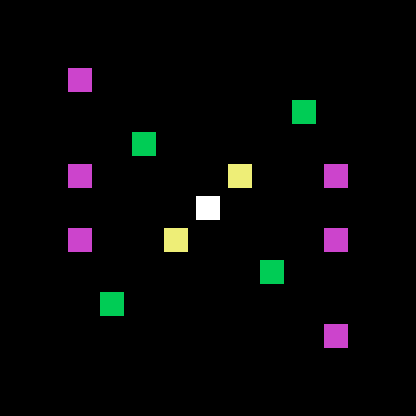
\includegraphics[width=1.3cm]{src/patterns/pixels/pixel_pattern5_7.png}%
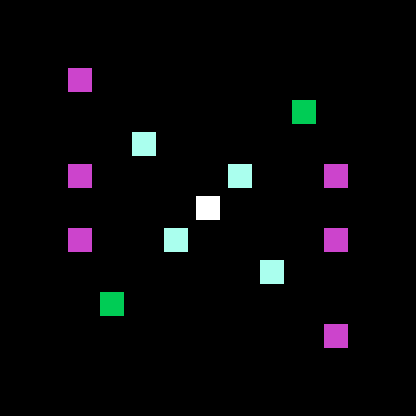
\includegraphics[width=1.3cm]{src/patterns/pixels/pixel_pattern5_8.png}%
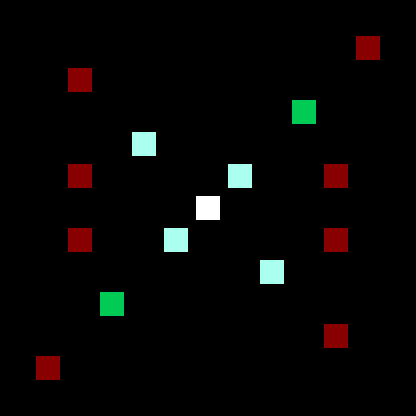
\includegraphics[width=1.3cm]{src/patterns/pixels/pixel_pattern5_9.png}%
} \\
        \midrule

        \makecell[l]{
\icode{.BYTE \$FB,\$05}\\
\icode{.BYTE \$05,\$FB}
} & \makecell[l]{
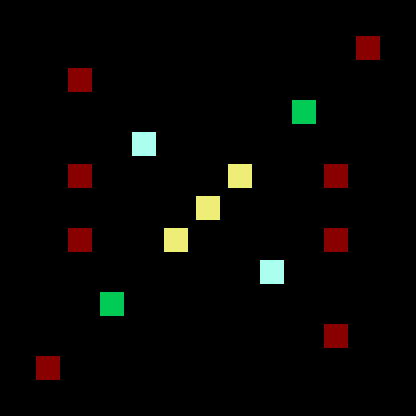
\includegraphics[width=1.3cm]{src/patterns/pixels/pixel_pattern5_10.png}%
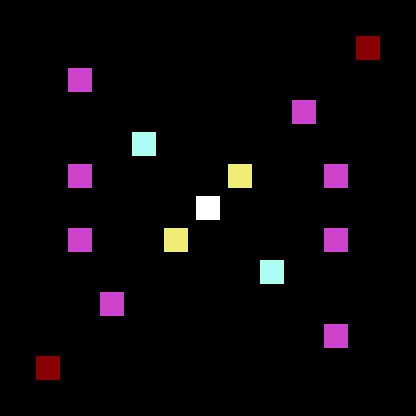
\includegraphics[width=1.3cm]{src/patterns/pixels/pixel_pattern5_11.png}%
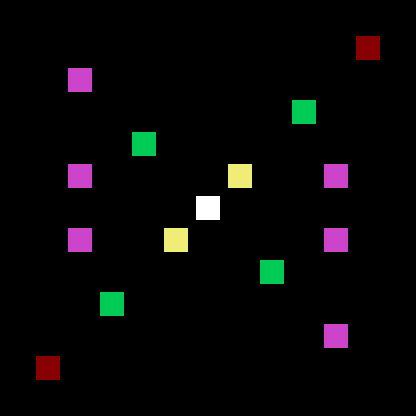
\includegraphics[width=1.3cm]{src/patterns/pixels/pixel_pattern5_12.png}%
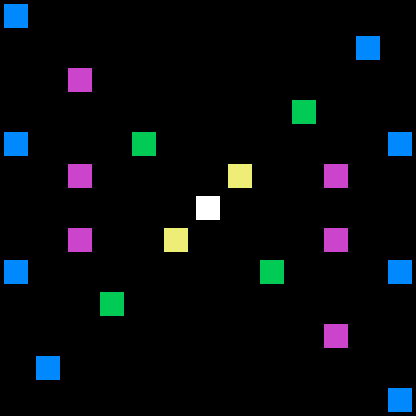
\includegraphics[width=1.3cm]{src/patterns/pixels/pixel_pattern5_13.png}%
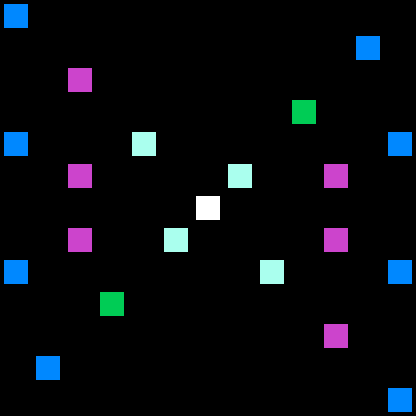
\includegraphics[width=1.3cm]{src/patterns/pixels/pixel_pattern5_14.png}%
} \\
        \midrule

        \makecell[l]{
\icode{.BYTE \$FA,\$06,\$FA,\$FA,\$06,\$06}\\
\icode{.BYTE \$FA,\$06,\$FE,\$02,\$FE,\$02}
} & \makecell[l]{
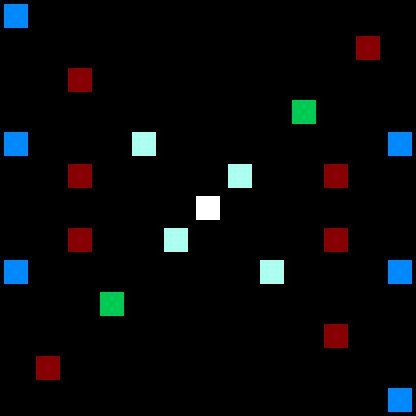
\includegraphics[width=1.3cm]{src/patterns/pixels/pixel_pattern5_15.png}%
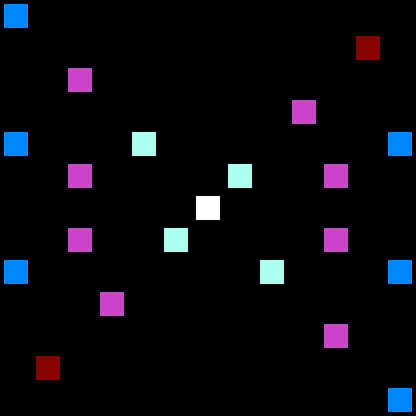
\includegraphics[width=1.3cm]{src/patterns/pixels/pixel_pattern5_16.png}%
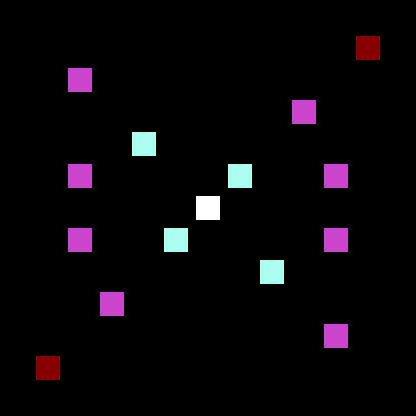
\includegraphics[width=1.3cm]{src/patterns/pixels/pixel_pattern5_17.png}%
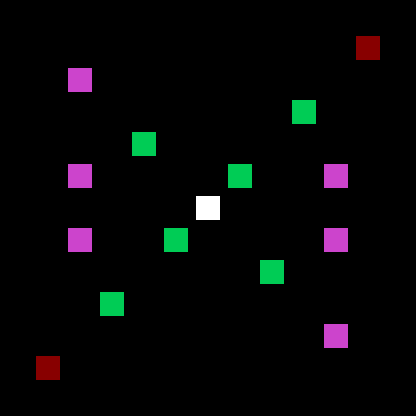
\includegraphics[width=1.3cm]{src/patterns/pixels/pixel_pattern5_18.png}%
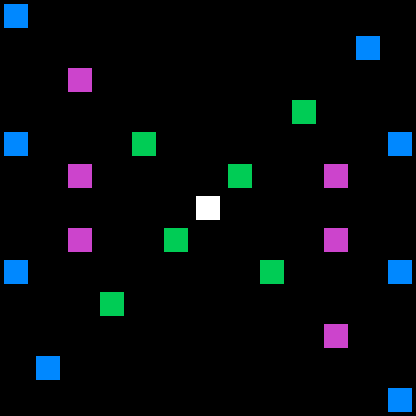
\includegraphics[width=1.3cm]{src/patterns/pixels/pixel_pattern5_19.png}%
} \\
        \midrule

        \makecell[l]{
\icode{.BYTE \$00}\\
\icode{.BYTE \$00}
} & \makecell[l]{
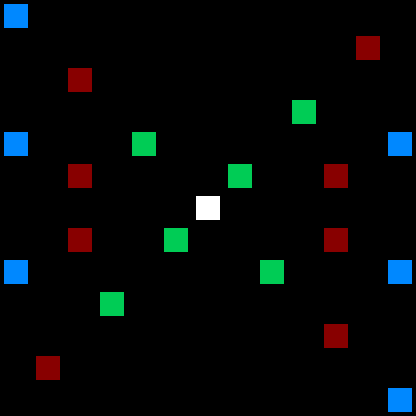
\includegraphics[width=1.3cm]{src/patterns/pixels/pixel_pattern5_20.png}%
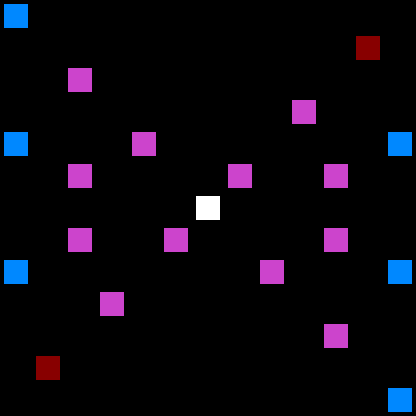
\includegraphics[width=1.3cm]{src/patterns/pixels/pixel_pattern5_21.png}%
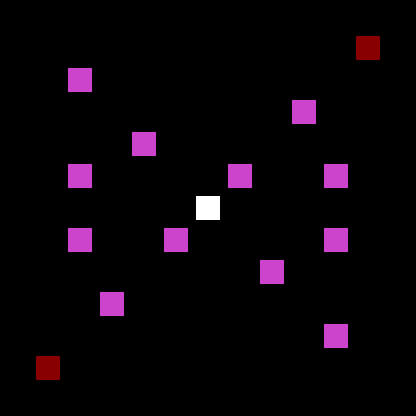
\includegraphics[width=1.3cm]{src/patterns/pixels/pixel_pattern5_22.png}%
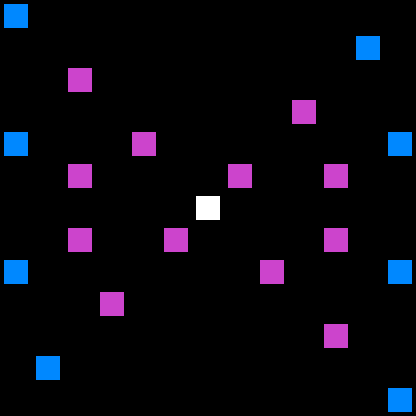
\includegraphics[width=1.3cm]{src/patterns/pixels/pixel_pattern5_23.png}%
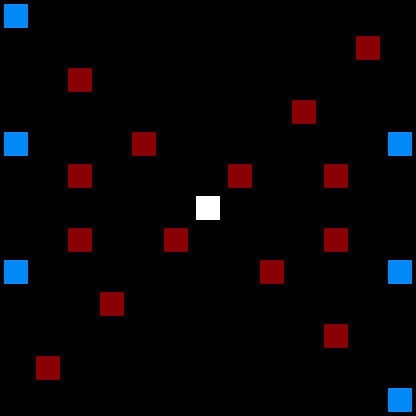
\includegraphics[width=1.3cm]{src/patterns/pixels/pixel_pattern5_24.png}%
} \\
        \midrule

      \end{tabular}
    \end{adjustbox}
  }\caption{The purpose of each of the oscillator values.}
\end{figure}
